\chapter{First search for eccentric spinning neutron star binary mergers}

%This chapter summarizes the search performed in the paper \cite{Dhurkunde:2023qoe}. We have targeted a previously unexplored region of the parameter space for search of eccentric binary systems. We did not find any new significant events, but explore upper limits for four different astrophysical models which have a wide range of astrophysical and physical implications.  

This chapter is a full reprint of \cite{Dhurkunde:2023qoe}, with some minor formatting, and an extra figure and a table. In this work we present our search results for eccentric spinning neutron star binaries from the third observing run of Advanced LIGO and Virgo. Using our search results we put state-of-art constraints for various astrophysical models and predict the capability of future observatories to determine the formation histories of compact binaries.  


\section{Introduction}

Gravitational-wave (GW) astronomy is becoming routine; nearly $100$ compact binary mergers have been observed to date \cite{Nitz:2021zwj,LIGOScientific:2021djp,Olsen:2022pin} using the Advanced LIGO  \cite{LIGOScientific:2014pky} and Advanced Virgo \cite{Acernese:2015gua} observatories. These observations have fueled interest in the long-standing question in astrophysics: \textit{how do compact binary systems form and evolve?} One class of models suggests these systems evolve as isolated stars in the field via common envelope \cite{Belczynski:2001uc, Mennekens:2013dja, Chu:2021evh}, stable mass transfer \cite{Klencki:2021hxe,vandenHeuvel:2017pwp} or via chemically homogeneous mixing \cite{Mandel:2015qlu, Marchant:2016wow}. Alternatively, they may be a result of a dynamical encounter of two or more separately evolved compact objects in dense environments such as globular clusters \cite{Vesperini:2010zi,Fragione:2018vty, Rodriguez:2017pec,Sedda:2020wzl}, nuclear star clusters \cite{Fragione:2018yrb, Wang:2020jsx}, young star clusters \cite{Banerjee:2020qub, Santoliquido:2020bry}, or active galactic nuclei \cite{Bartos:2016dgn, Tagawa:2020qll}.
Current GW catalogs suggest that multiple formation pathways contribute to the population of binary black hole (BBH) mergers in the Universe rather than a single preferred channel \cite{Zevin:2020gbd,KAGRA:2021duu}. However, there is an insufficient number of observed neutron star binaries (BNS or NSBH) to determine if there is a preference for a single dominant channel or several competing channels present~\cite{KAGRA:2021duu,Belczynski:2017mqx}.

%observations using GWs \cite{Nitz:2021zwj,LIGOScientific:2021djp,Olsen:2022pin} or radio pulsars \cite{Tauris:2017omb,Ozel:2015fia} 

Each formation channel makes distinct predictions for the distribution of binary properties, e.g. masses, spins, eccentricity and merger rate~\cite{Mandel:2021smh}. Distinguishing these channels could be done by careful comparison of large number of detected events or by identifying rare events with properties that are unique to a specific channel \cite{Zevin:2020gbd,Zevin:2021rtf,Dhurkunde:2022aek}. Orbital eccentricity carries a strong signature of a binary's evolutionary history: although the initial eccentricity of a binary is close to unity due to asymmetrical supernovae kicks  \cite{Hobbs:2005yx, Verbunt:2017zqi}, the evolution of eccentricity is influenced by the binary's surrounding environment.  In field binaries, energy dissipation solely occurs through GW emission, resulting in a swift reduction in eccentricity as the system evolves in frequency -- becoming nearly negligible when GW frequency reaches the sensitive band of current GW observatories (e.g 10 Hz) \cite{Peters:1964zz}. Whereas, in dense environments, angular momentum exchanges with a third compact object via the Lidov-Kozai (LK) mechanism \cite{LIDOV1962719,Kozai:1962zz, Antognini:2015loa} can result in sustained non-negligible eccentricities at GW frequencies sensitive to current detectors. 

\begin{sidewaysfigure}
        \centering
    \includegraphics[width=\textwidth]{figures/ecc_search/eccentricity_dist.png}
    \caption{Distribution of orbital eccentricities (left column) for different formation models \cite{Belczynski:2017mqx, Sedda:2020wzl,Trani:2021tan,Fragione:2018yrb} at the time of formation of compact binaries (green) and when the dominant-mode of GW frequency reach 10 Hz (pink). All four models predict mergers to born with high natal eccentricities. Considering energy loss via GW only, eccentricity is quickly radiated away as evident by the clear shift in the distributions for the isolated BNS channel \cite{Belczynski:2017mqx} and for NSBH mergers in globular clusters \cite{Sedda:2020wzl}. The nuclear cluster \cite{Fragione:2018yrb} and hierarchical triples \cite{Trani:2021tan} models describe eccentricity enhancing scenarios where NSBH binaries can retain non-negligible eccentricities at 10 Hz. We also show the chirp mass distribution predicted by each model in the second column and the estimated chirp masses of the observed BNS (GW170817, GW190425) and NSBH (GW200105, GW200115) events.}
    \label{fig:eccentricity-dist}    
\end{sidewaysfigure}

We highlight four formation scenarios in Fig. \ref{fig:eccentricity-dist} as a fiducial comparison \cite{Belczynski:2017mqx,Sedda:2020wzl,Trani:2021tan,Fragione:2018yrb}. We have considered two models without eccentricity enhancing mechanisms -- one for isolated BNS binaries \cite{Belczynski:2017mqx} and for NSBH systems in globular clusters \cite{Sedda:2020wzl}. We also study two models with eccentricity inducing mechanisms -- NSBH systems in hierarchical triples \cite{Trani:2021tan} and in nuclear clusters \cite{Fragione:2018yrb}. In models influenced by the LK mechanism, up to $80\%$ of the systems could possess eccentricity $e_{10} \geq 0.01$ (eccentricity at dominant-mode gravitational-wave frequency of 10 Hz ($e_{10}$)) \cite{Hamers:2019oeq, Fragione:2018yrb,Trani:2021tan, Silsbee:2016djf,Rodriguez:2018jqu}, and in the absence, only up to $5\%$ of the sources exceed this eccentricity \cite{Sedda:2020wzl, Belczynski:2017mqx}. Observation of an eccentric system would clearly indicate the presence of a dynamical channel. Even a null detection would allow us to put tighter constraints on the predicted merger rates which are highly sensitive to the unconstrained parameters describing physical process such as common-envelope evolution \cite{Marchant:2021hiv,Santoliquido:2020bry, Baibhav:2019gxm}, natal supernovae kicks \cite{Belczynski:2001uc,Hamers:2019oeq,Trani:2021tan,Santoliquido:2020bry,Silsbee:2016djf, Richards:2022fnq, Baibhav:2019gxm} or dynamics of dense environments \cite{Fragione:2018yrb,Ford:2021kcw,Petrovich:2017otm}. 


Four neutron star binary mergers have been observed to date: two BNS mergers GW170817 \cite{LIGOScientific:2017vwq} and GW190425 \cite{LIGOScientific:2020aai} and two potential NSBH mergers GW200105 and GW200115 \cite{LIGOScientific:2021qlt}. All of these binaries were found using searches that only model quasi-circular binary orbits \cite{Messick:2016aqy,Aubin:2020goo,Allen:2005fk,Usman:2015kfa}. If neutron star binaries have sufficiently high eccentricities, they would be missed by these searches \cite{Huerta:2013qb,Lenon:2021zac}.   The two BNS mergers have eccentricities limited to $e_{10} \leq 0.024$ and $e_{10} \leq 0.048$ for GW170817 and GW190425, respectively \cite{Lenon:2020oza}. 
% need somethign more after this sentence
%The measurement of a nonzero eccentricity of a binary merger would be a smoking gun for a dynamical formation channel. 
In this Letter, we report the results for the first search for NSBH and the latest from BNS aligned-spin eccentric systems. A previous search for BNS mergers in the data from Advanced LIGO and Virgo's second observing run used a narrower range of binary masses (shown in Fig. \ref{fig:search_region}) and did not account component-object spins \cite{Nitz:2019spj}. Searches for eccentric subsolar binaries has also been performed \cite{Nitz:2021vqh,Wang:2021qsu}. Only unmodeled searches have been performed for eccentric BBH systems ~\cite{LIGOScientific:2019dag, LIGOScientific:2023lpe, Pal:2023dyg}. While these searches did not yield any new candidates, they constrained the local merger rate to be less than: $1700$ mergers $\text{Gpc}^{-3} \text{Yr}^{-1}$ for BNS systems with $e_{10} \leq 0.43$ and $0.33$ mergers $\text{Gpc}^{-3} \text{Yr}^{-1}$ for BBH systems with total mass $M \in [70M_{\odot},200M_{\odot}]$ and $e_{15} < 0.3$ at 90\% confidence. In addition, radio pulsar surveys have discovered over twenty BNS systems exhibiting a broad range of eccentricities between 0.06 and 0.8 \cite{Bernadich:2023uru} (see Table I). These observations constrain the BNS local merger rate to $293^{+222}_{-103}$ $\text{Gpc}^{-3} \text{Yr}^{-1}$.


We do not find any new mergers in the public data from the third observing run (O3) of Advanced LIGO and Advanced Virgo observatories. We use our observations and the capabilities of future observatories to constrain an isolated BNS model and three different models for NSBH mergers in globular clusters, nuclear clusters and hierarchical triples: our observations restrict the rate of mergers for BNS binaries to be less than $\sim 150$ mergers $\text{Gpc}^{-3}\text{Yr}^{-1}$ and less than $\sim $ 50 -- 100 mergers $\text{Gpc}^{-3}\text{Yr}^{-1}$ for NSBH binaries at 90\% confidence. These constraints assume that the prior observed BNS and NSBH mergers are from alternate formation channels. Assuming they are from one or more of the channels we consider, the measured rate would be consistent given the sparsity of observations. We predict the capabilities of improved second generation and upcoming third-generation GW observatories to use eccentric binary observations to constraint formation models. We find that a network of Cosmic Explorer (CE) (40 km) + CE (20km) observatories will detect the majority of sources from each of these models and could determine that a subset of the population have non-negligible eccentricities. A network of three $\text{A}^{\#}$ observatories would require at least $\sim$ two years of observation to detect a non-negligible eccentric NSBH merger from hierarchical triples or nuclear clusters.    

\begin{figure}
    \centering
    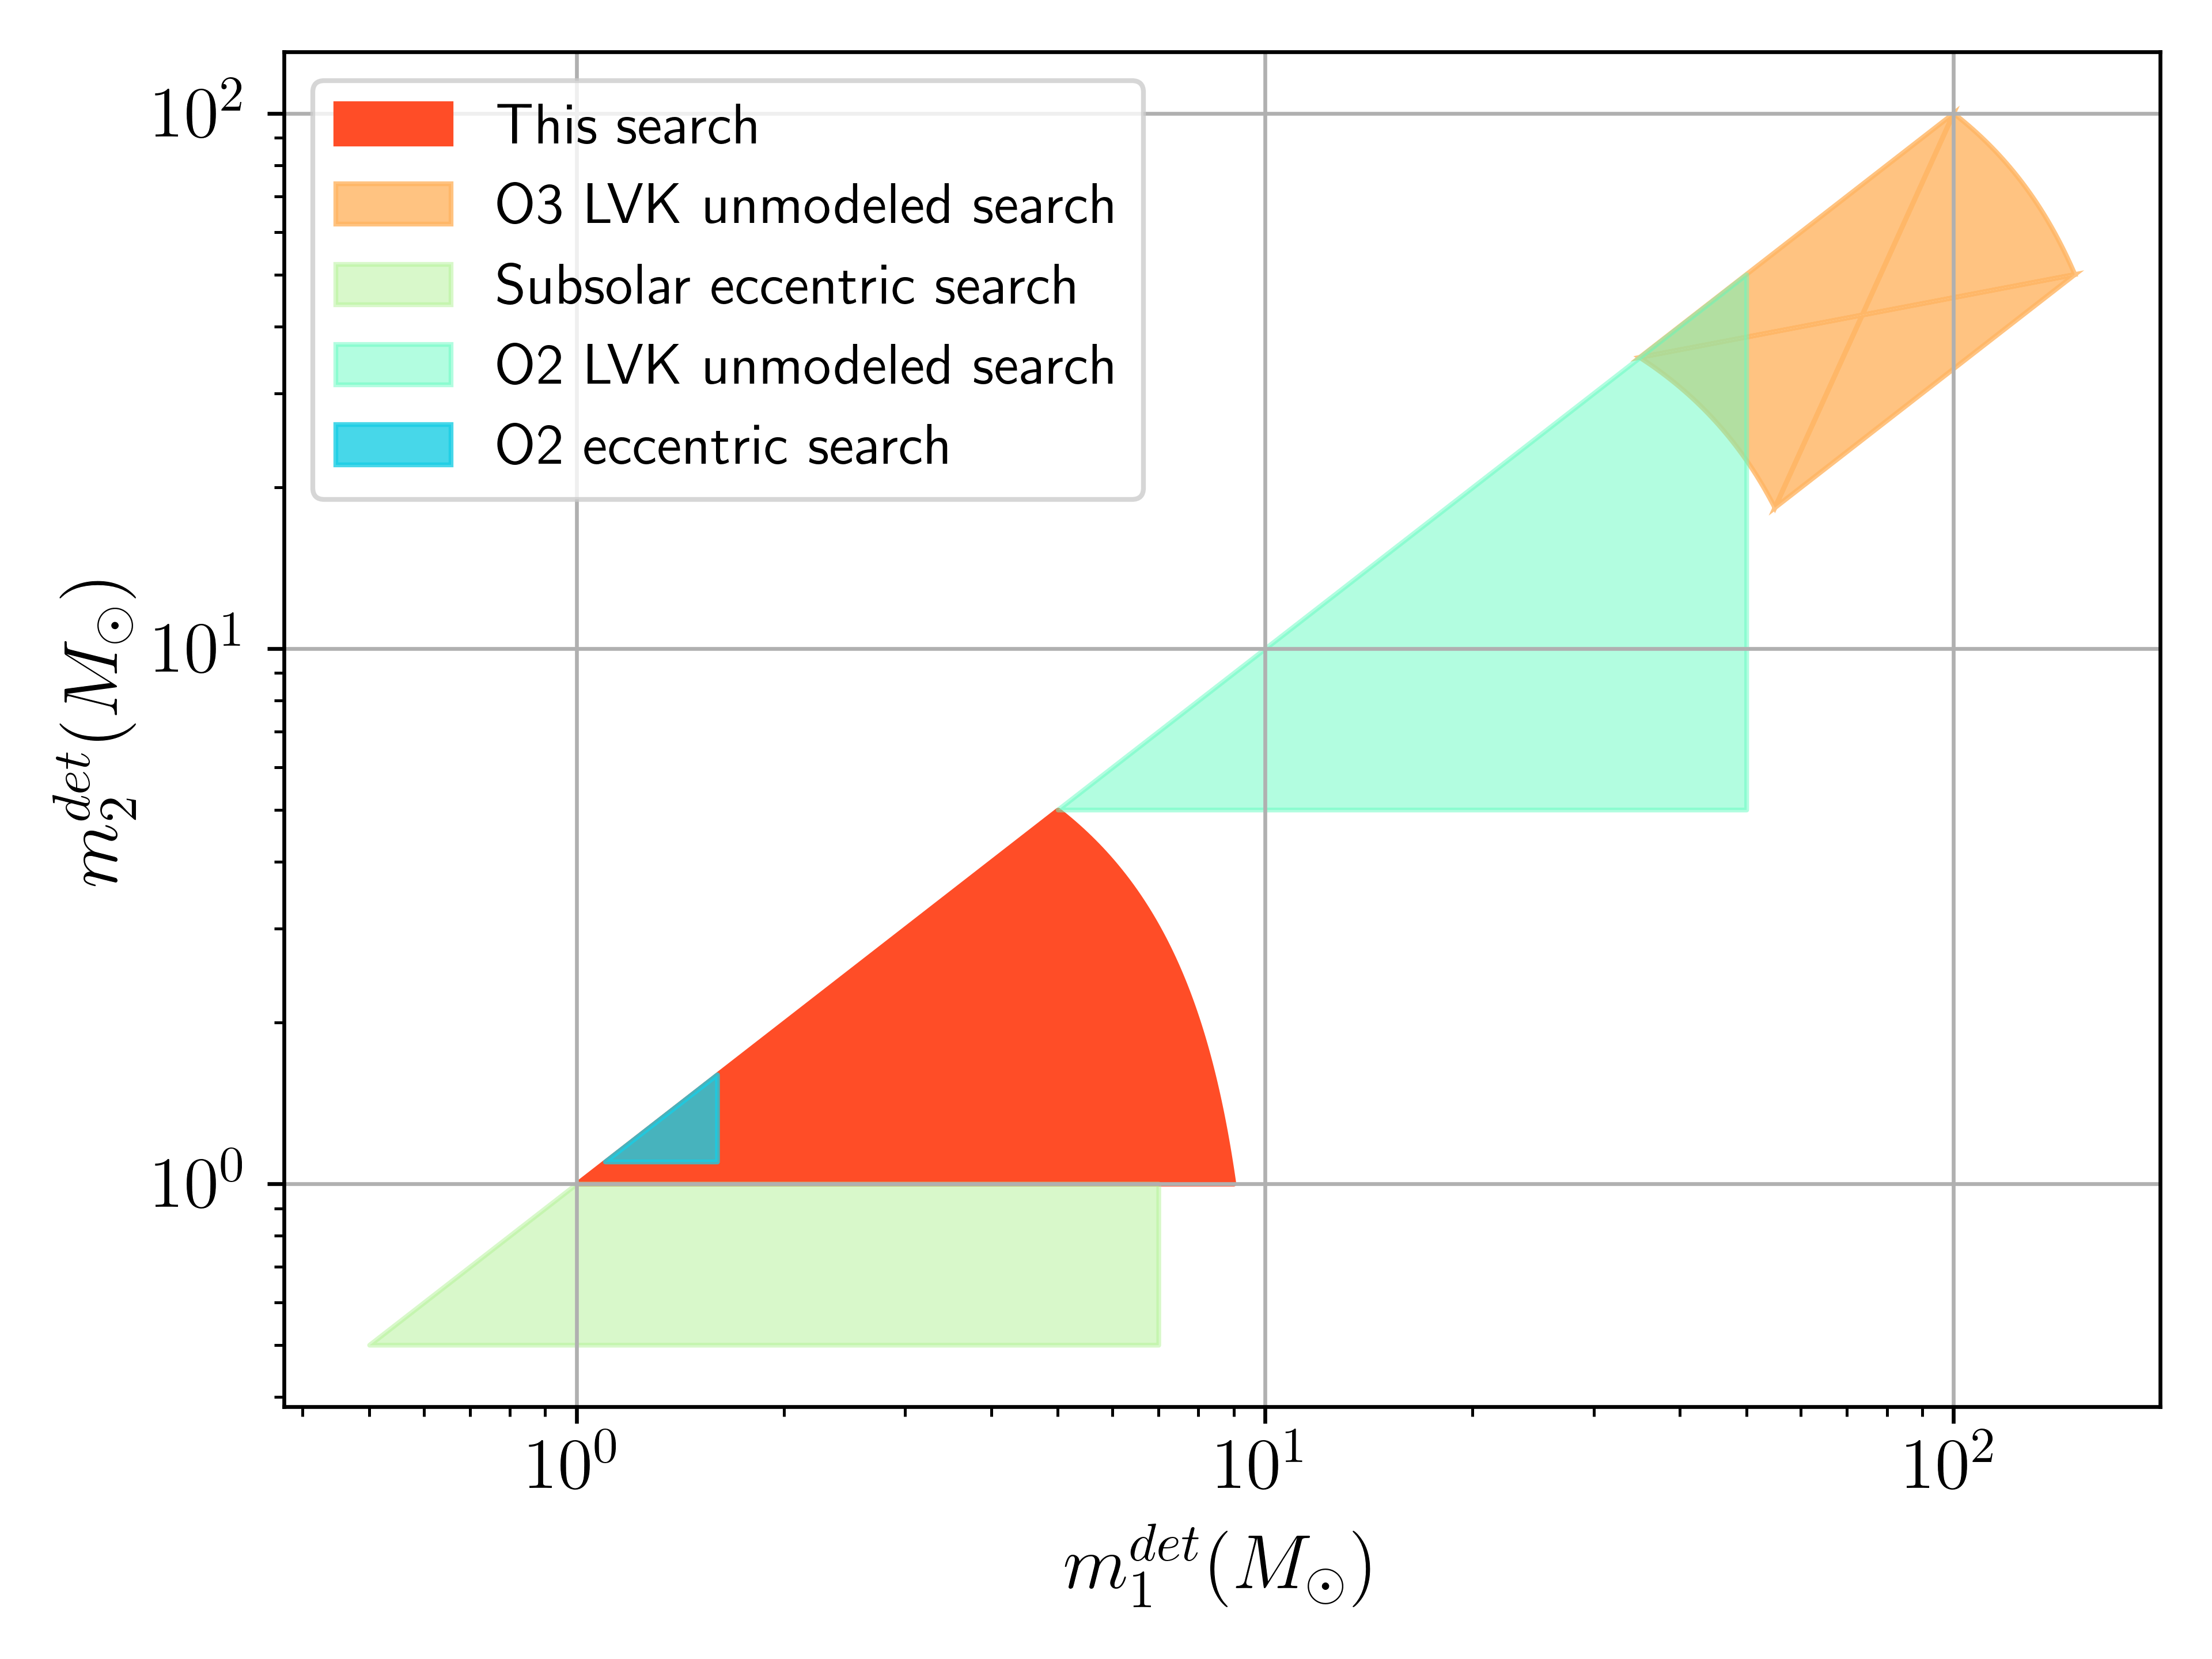
\includegraphics[width=\textwidth]{figures/ecc_search/Search_region.png}
    \caption{ Target regions of the various eccentric searches performed to date \cite{Nitz:2019spj,Nitz:2021vqh,LIGOScientific:2019dag,LIGOScientific:2023lpe} as a function of detector-frame masses ($m_1^{det}-m_2^{det}$). No prior searches have been explored for NSBH systems or BNS systems with spins. The prior search for BNS systems was restricted to a narrower region of masses and eccentricities ($e_{10} \leq 0.43$) and did not include spins \cite{Nitz:2019spj}. We search for spin-aligned neutron star binaries (BNS + NSBH) with eccentricities $e_{10} \leq 0.46$. The only searches for BBH sytems are unmodeled searches \cite{LIGOScientific:2019dag,LIGOScientific:2023lpe} and show the regions used to report their upper limits. The previous search for non spinning subsolar binaries restricted the eccentricities to $e_{10} \leq 0.3$ \cite{Nitz:2021vqh}.}
    \label{fig:search_region}
\end{figure}


\section{Search description and observational results}
To search for eccentric binaries, we use the PyCBC toolkit to perform a template-based matched filtering analysis to find modeled GW signals in the interferometric data \cite{Usman:2015kfa,Nitz:2017svb}. GW candidates are identified by finding peaks of the signal-to-noise (SNR) time-series, mitigating non-Gaussian noise artefacts, and checking the consistency of the data and astrophysical sources between each detector~\cite{Allen:2004gu, Nitz:2017lco,Davies:2020tsx}. Taking into account these factors and the empirically measure noise distribution, each candidate is assigned a ranking statistic value \cite{Nitz:2017svb, Davies:2020tsx, Was:2009vh}.

We search for neutron star binaries using a bank of modeled waveforms (templates) generated using a stochastic placement method \cite{Harry:2009ea,Babak:2008rb}. Our   
search region is described by five binary parameters: detector-frame component masses ($m_1^{det}, m_2^{det}$) ranging from [1.0, 9.0] $M_{\odot}$ with cutoff on total mass $M \leq 10 M_{\odot}$, $z-$ component of the individual spins ($\chi_{1z}, \chi_{2z} \in [-0.1, 0.1]$), eccentricity $e_{20}$ at 20 Hz $\in [0, 0.28]$, and an additional source orientation parameter $l$ related to the position of the periapsis. Our eccentric bank contains $\sim$ 6 million templates which is roughly two orders of magnitude larger than an equivalent bank for quasi-circular binaries. To model the GW signals, we use TaylorF2e inspiral only waveform model \cite{Moore:2016qxz} which accounts for eccentricity corrections to the aligned-spin quasi-circular TaylorF2 model \cite{Buonanno:2009zt}. Eccentricity causes phase and amplitude modulations of the GW signal, as shown in the Fig. (\ref{fig:ecc-WF}). Our search is reliably performed using only the inspiral part of the signal, since the merger falls outside the sensitive band of the current detectors. 

\begin{figure}
    \centering
    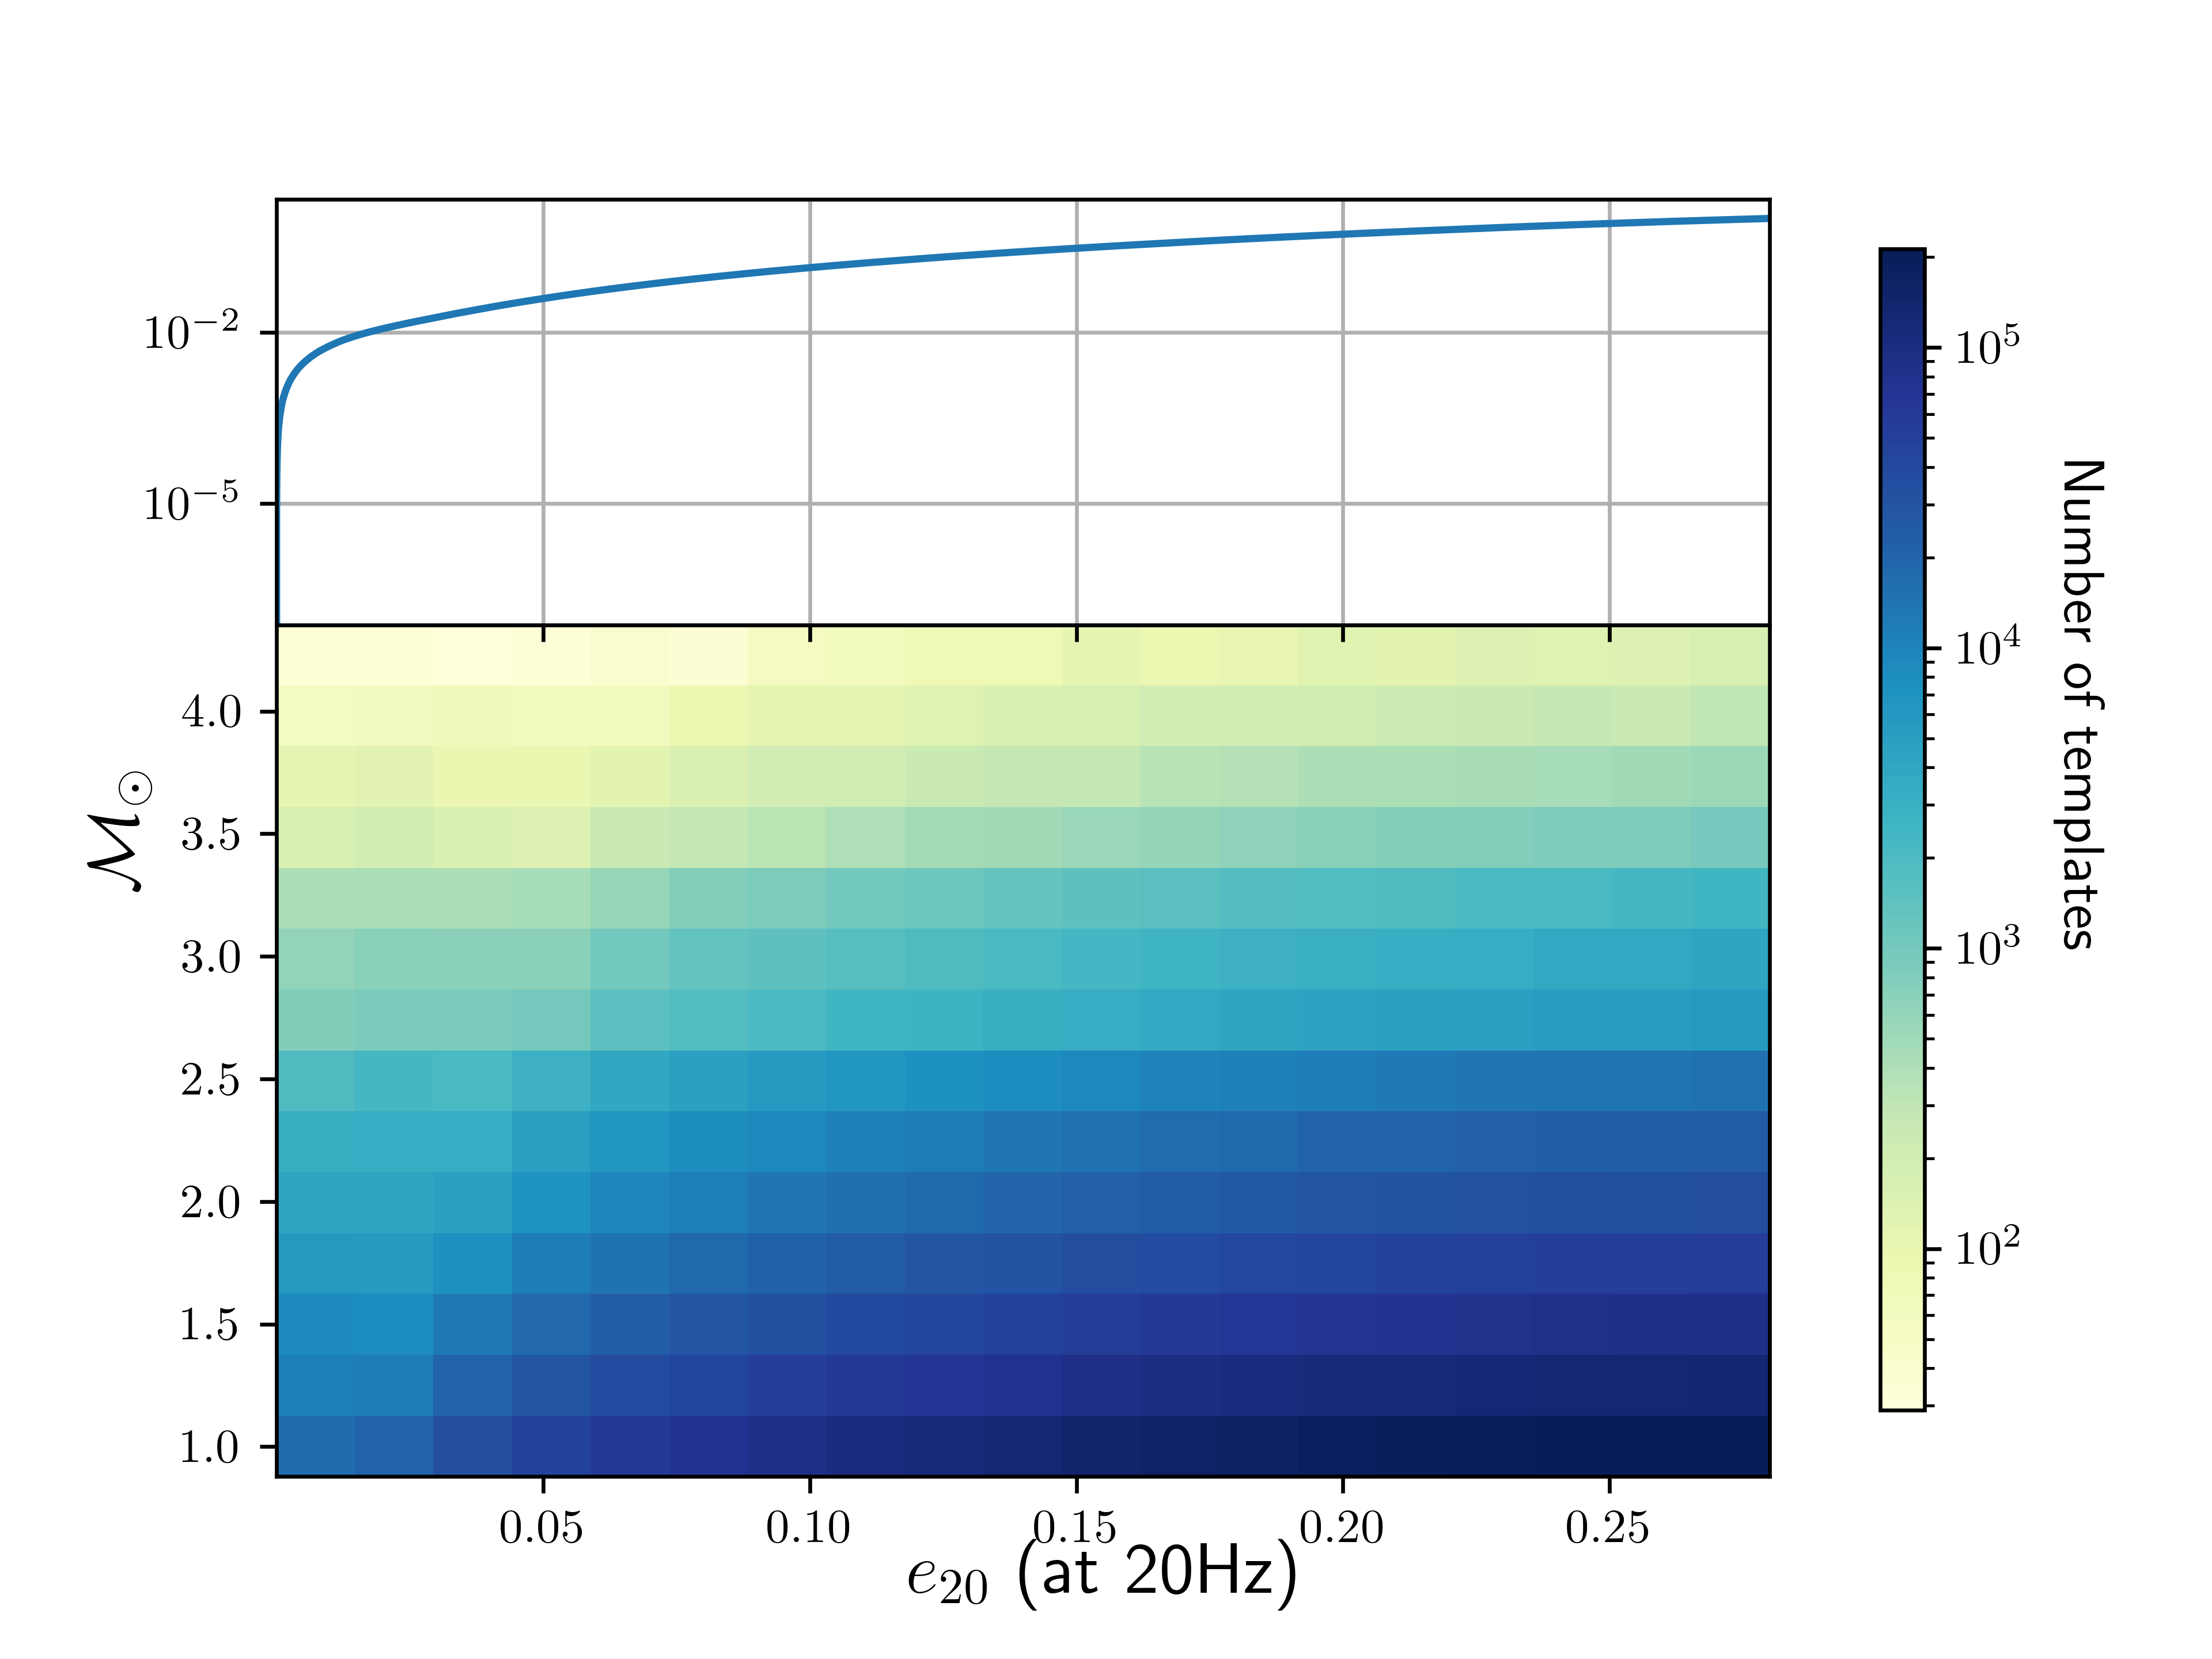
\includegraphics[width=\textwidth]{figures/ecc_search/bank_density.png}
    \caption{Our eccentric template bank as a function of the eccentricity at 20 Hz ($e_{10}$) and chirp mass. In the bottom panel we show the two dimensional binned histograms with the colorbar indicating the number of templates in each bin. The number of templates required to cover the parameter space increases with eccentricity -- our template bank contains $\sim 6$ million templates, an order of magnitude larger than an equivalent bank for circular binaries. In the top panel we show the cumulative distribution of templates as the function of eccentricity.}
    \label{fig:ecc-bank}
\end{figure}

\begin{figure}
    \centering
    \includegraphics[width=\textwidth]{figures/ecc_search/eccentric-wf.png}
    \caption{Effect of orbital eccentricity on the GW signal from $(10-10)M_{\odot}$ binary, two different scenarios are shown -- circular binary (pink) and eccentricity at 20 Hz ($e_{20} = 0.5$) (green). Eccentricity causes phase and amplitude modulations of the waveform. Eccentric binary radiates energy much quicker than a circular system, as evident by the shorter eccentric waveform.}
    \label{fig:ecc-WF}
\end{figure}


We search the O3 public Advanced LIGO and Virgo datasets using broadly the same search methods as \cite{Nitz:2021zwj}. O3 was divided into two parts -- O3a and O3b, comprising in total of $\sim 249$ days of coincident time when at least two observatories were in operation. Our search does not find any new significant GW candidates and recovered the previously reported multi-detector NSBH event GW200115 with high significance. The most significant candidate has a FAR of about 1 per year, consistent with the null hypothesis based on the observation duration. We show in the table \ref{tab:significant-events} the three most notable candidates, the list of top candidates, the template parameters associated with each candidate, and the configuration files necessary to reproduce the analysis are available in our data release~\cite{github}.  

\begin{table}[H]
    \centering
    \begin{tabular}{ccccccc}
        \hline
        \hline
         GPS time &  IFAR & $m_1$ & $m_2$ & $e_{10}$ & $\chi_{1z}$ & $\chi_{2z}$\\
         & (Yr)& $(M_{\odot})$ & $(M_{\odot})$ & & & \\
         \hline
         1247741648.397 & 1.02 & 1.56 & 1.02 & 0.36 & 0.04 & -0.07 \\
         1257948134.021 & 0.82 & 1.19 & 1.13 & 0.24 & -0.01 & -0.03 \\
         1265599361.194 & 0.43 & 2.95 & 1.03 & 0.22 & 0.05 & -0.08 \\
        \hline
    \end{tabular}
    \caption{Table of top three significant events from our search, sorted by the inverse false alarm rates (IFARs). The global positioning system (GPS) time of each candidate, the component mass $m_{1/2}$ (detector frame), eccentricity at $e_{10}$, and component spins $s_{1z/2z}$ of the template chosen by the search are shown.}
    \label{tab:significant-events}
\end{table}

We demonstrate the sensitivity of our search by the ability to recover a population of simulated sources as a function of luminosity distance $d_L$ for fixed chirp mass and orbital eccentricity $e_{10}$ averaged over sky locations and orientations. We generate the signals using the TaylorF2e approximant. Fig. \ref{fig:sensitive-dist} shows the average sensitive distance as a function of $e_{10}$ for four different values of $\mathcal{M}_c$. It is evident from the plot that sensitive distance scales linearly with the chirp mass and has a weak dependence on the eccentricity. As a comparison the sensitive distance for a fiducial $\mathcal{M}_c = 1.22 (1.4-1.4 M_{\odot})$ is improved from roughly 90 Mpc to 125 Mpc from O1/O2 to O3 run due to improvements in the current detectors. We point out the drop in sensitivity towards higher eccentricity because this region is outside of our search parameter space. 

\begin{figure}[h]
    \centering
    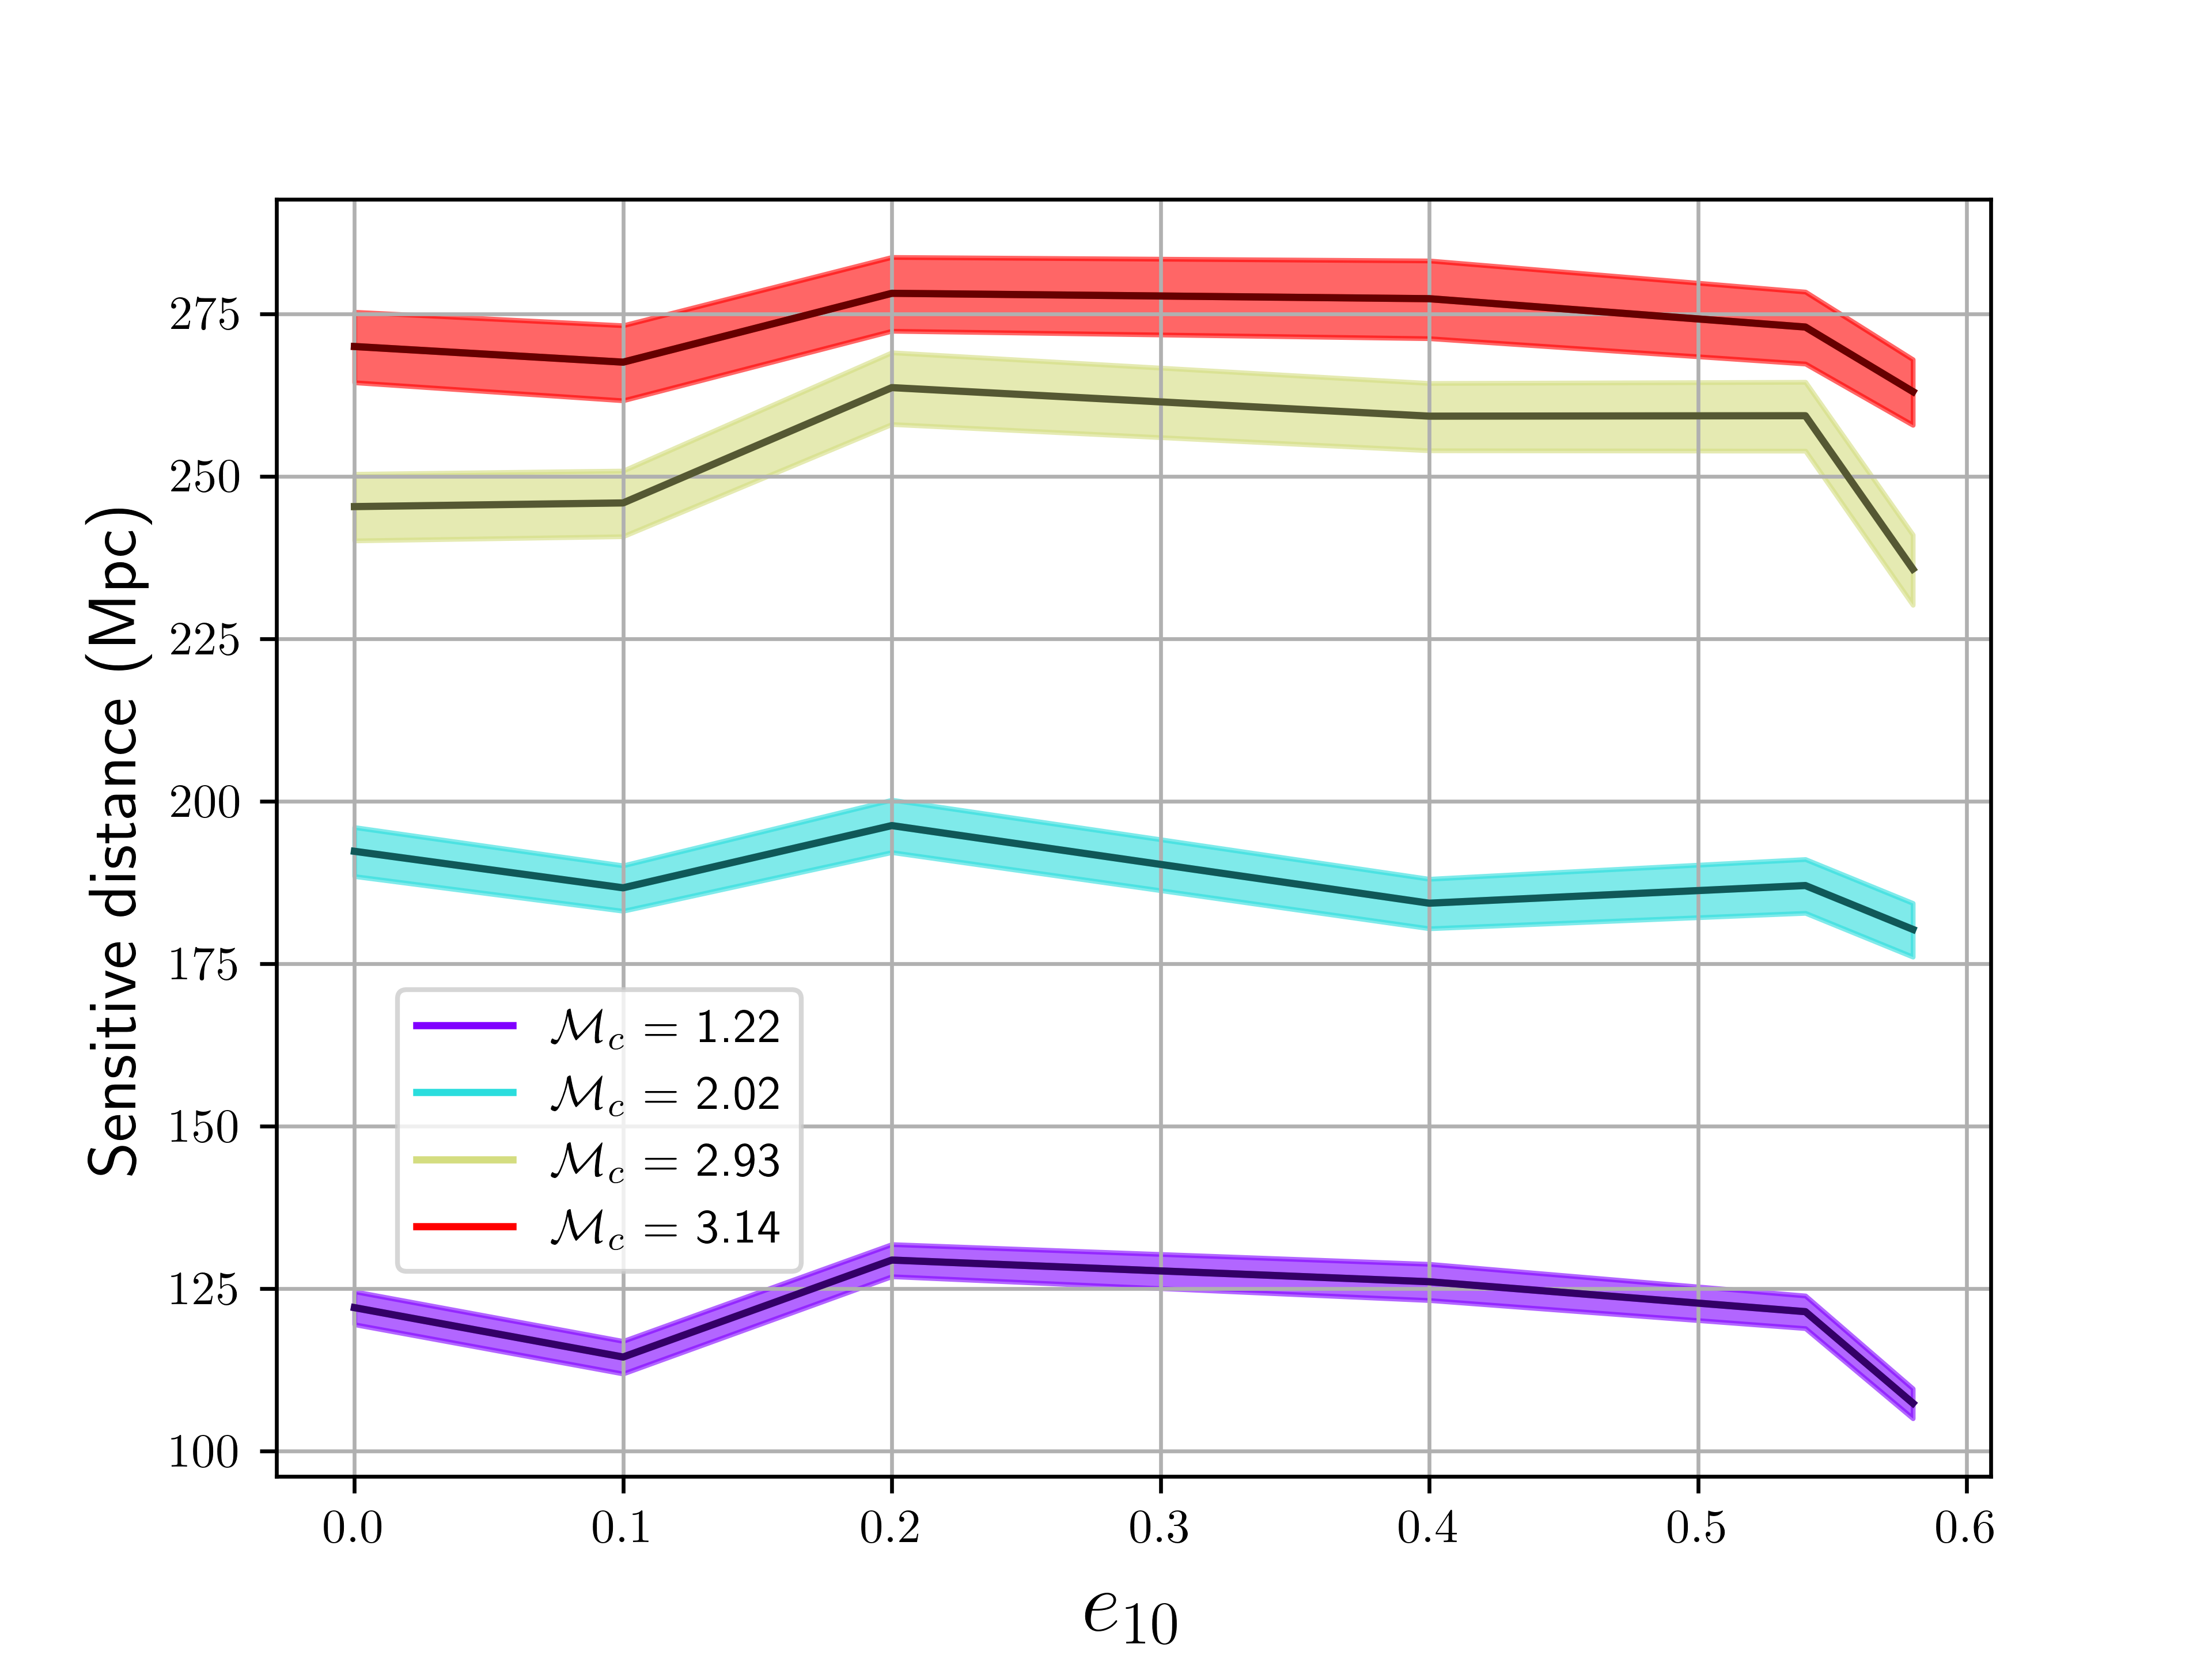
\includegraphics[width=\linewidth]{figures/ecc_search/SENS_DIST_ecc.png}
    \caption{Sensitive distance as a function of $e_{10}$ for systems with four different fixed $\mathcal{M}_c$ averaged over sky and orientation (Recast the axis to 10 Hz). The sensitive distance of our search is $\sim 1.3 \times$ better than previous eccentric BNS search due to the improvements in detector from O2 to O3. We remark that the sensitive distance increases with the chirp mass and varies weakly with eccentricity.}
    \label{fig:sensitive-dist}    
\end{figure}

\section{Constraining population models}

For a given astrophysical model with a merger rate density $\mathcal{R}(\theta, z)$, the expected number of detections within an observation period $T_{obs}$ is 
\begin{align}
    N_{detected} & = T_{obs} \int \int \mathcal{R}(\theta,z) f(\theta,z) \dfrac{dV_c}{dz}\dfrac{1}{1+z} d\theta dz ,
    \label{Eq:expected-detections}
\end{align}
where $p(\theta)$ is the distribution function of the binary parameters ($\theta$) predicted by an astrophysical model, $dV_c/dz$ is the differential co-moving volume and $f(z,\theta)$ is the probability of detecting a merger with $\theta$ parameters at a redshift $z$. We can constrain the local merger rate using the lack of observations: if we assume a Poisson distribution of observed mergers, then the 90\% confidence limit $R_{90}^{local}$ corresponds to a local merger rate when the expected number of detections is $\sim 2.3$ \cite{Biswas:2007ni}.


Upper limits are obtained by estimating the expected number of detections $N_{detected}$ (Eq. \ref{Eq:expected-detections}) via a Monte Carlo (MC) integration scheme for a synthetic population of mergers with binary parameter distributions predicted by the respective models \cite{Tiwari:2017ndi}. For a search, the detection probabilities can be estimated by using the search to detect simulated sources injected into the data. In our simulations, we assume the merger rate density follows the star formation rate \cite{Madau:2016jbv} convolved with the inverse time-delay distribution, same as the method used in \cite{Zhu:2020ffa, Wu:2022pyg}. The injection results from our search and the codes to estimate the observational limits are available as a part of our data release \cite{github}.  


\begin{sidewaysfigure}
    \centering
    \includegraphics[width=\textwidth]{figures/ecc_search/expected_ranges.png}
    \caption{ Predicted and observed constraints on the local merger rate for various populations of BNS and NSBH sources \cite{Belczynski:2017mqx, Sedda:2020wzl,Trani:2021tan,Fragione:2018yrb}. Assuming the observed neutron star binaries are part of the channels we considered, our measured rate (horizontal orange bars) is consistent with the observed rates in existing GW catalogs \cite{Nitz:2021zwj,LIGOScientific:2021djp,Olsen:2022pin}. The observational constraints assuming a null detection from our search for 249 days of observation is shown as blue (hatched) region. Predicted constraints for an idealized search are shown for O3 (blue), three $\text{A}^{\#}$ (green) and CE (40km) + CE (20km) (pink) for an year of observation. In an idealized search signals from high mass mergers can all be detected if they exceed a network SNR of 10: achieving this, our search constraints would be up to $5\times$ tighter reaching the idealized O3 limits (solid blue line). Next generation detectors will detect tens to hundreds of binaries, but not all would have sufficiently high eccentricities to be distinguished from non-eccentric binaries. When focusing on systems where $e_{10}\geq0.01$, the upper limits deteriorate inversely to the fraction of sources predicted by each model, affecting up to 80\% of NSBH systems from hierarchical triples or nuclear clusters. A fixed threshold does not capture the varied ability of different observatory networks to measure eccentricity. We further define a system with a measurable nonzero eccentricity if a non-eccentric model can be ruled out at the 90\% credible level. Using our predictions we can estimate the time required for an eccentric merger observation; the hierarchical triples model predicts a maximum merger rate of 0.34 $\text{Gpc}^{-3}\text{Yr}^{-1}$ and the $\text{A}^{\#}$ limit for systems with measurable eccentricity is 0.74 $\text{Gpc}^{-3}\text{Yr}^{-1}$, this gives an expected 2.2 years of observations with $\text{A}^{\#}$ for an eccentric NSBH merger observation. Three $\text{A}^{\#}$ will require 2 -- 100 years of observation to detect an eccentric NSBH merger for the range of models. CE will be able to detect mergers from every model and able to determine the eccentricity of tens to hundreds of binaries. This is even the case for isolated BNS mergers.
    } 
    \label{fig:time-requirement}    
\end{sidewaysfigure}

%%%%% Astrophysical constraints
\section{Astrophysical implications} 

We investigate how our observational results and the capability of future detectors can constraint four different astrophysical models: three dynamical pathways for NSBH systems within nuclear clusters \cite{Fragione:2018yrb}, globular clusters \cite{Sedda:2020wzl}, and hierarchical triples \cite{Trani:2021tan}, and a BNS formation model in the field \cite{Belczynski:2017mqx} to contrast the two major types of channels. The predicted merger rates of these models are shown in Fig. \ref{fig:time-requirement}. We constrain the local merger rate to be less than 150 $\text{Gpc}^{-3}\text{Yr}^{-1}$ (isolated BNS), 50 $\text{Gpc}^{-3}\text{Yr}^{-1}$ (NSBH in globular clusters), 100 $\text{Gpc}^{-3}\text{Yr}^{-1}$ (NSBH in hierarchical triples) and 70 $\text{Gpc}^{-3}\text{Yr}^{-1}$ (NSBH in nuclear clusters) under the assumption of non-detection from these channels. We also measure the rate of neutron star binaries from these models, assuming all prior observations are associated with each channel; these are consistent due to the lack of observations to date. Clearly, current GW observatories cannot constrain the dynamical formation models we have considered. 
%If we were to detect a highly eccentric merger it would necessitate a channel that can produce high eccentricities. 

Improved second generation and upcoming third generation observatories are expected to be a factor of a few and  more than an order of magnitude more sensitive than the current ones, respectively \cite{Asharp_sensitivity, CE_sensitivity}. Third generation detectors will be sensitive to the majority of neutron star binaries in the Universe. So the question arises: \textit{ To what extent can future observatories determine the formation history of neutron star binaries?} We predict how well upcoming second and third generation observatories will be able to constrain these models using an idealized search. We investigate constraints on the local merger rate for two networks (shown in Fig. \ref{fig:time-requirement}) -- one consisting of three $\text{A}^{\#}$ observatories and another composed of CE (40km) + CE (20km) using their expected noise curves \cite{Asharp_sensitivity, CE_sensitivity}. Furthermore, we have constraints for networks involving A+ and/or Einstein Telescope (ET) which are not presented here but are available in our data release \cite{github}. In agreement with \cite{Baibhav:2019gxm}, we find that CE will be able to detect majority of sources from each model. While current detectors may require up to $\mathcal{O}(10^3)$ years of observation to observe mergers from the considered dynamical formation models, three $\text{A}^{\#}$ observatories would begin detecting events from the most optimistic of these channels in roughly two years and CE (40km) + CE (20km) with a few days of observation.  
 
%Even when we are able to potentially observe binaries from each formation channel, only a fraction of binaries have sufficiently high eccentricities to distinguish them from non eccentric binaries: observations from future observatories may not be convincingly attributed to dynamical channels unless they have high eccentricity. 
Even though we can observe binaries from various formation channels, only those with high eccentricities can be clearly differentiated from non-eccentric binaries. Future observatory observations might struggle to confidently attribute binaries to dynamical channels unless they exhibit high eccentricity. To elucidate this, we show the population constraints for a fixed eccentricity threshold of $e_{10} \geq 0.01$ in Fig.~\ref{fig:time-requirement}. The limits for a fixed threshold scales inversely to the predicted fraction of systems satisfying this threshold: limits for mergers with $e_{10} \geq 0.01$ for NSBH in hierarchical triples or nuclear cluster models are worse only by a few factor due to large fraction of such sources predicted (see Fig. \ref{fig:eccentricity-dist}). 

The ability to measure eccentricity depends on the properties of a binary and the  \cite{Lower:2018seu} capabilities of a detector network, which a fixed threshold cannot capture -- we assess the potential of future observatories to measure eccentricity for each binary in our simulated population models. We determine the ability of a particular type of source to have non zero eccentricity using a simplified Bayesian analysis employing a Markov Chain Monte Carlo (MCMC) sampling scheme. We deem a source to have measurable eccentricity if at the 90\% credible level we can rule out the quasi-circular binary hypothesis. We find the threshold $e_{10} \geq 0.01$ falls short for measuring eccentric neutron star binaries with three $\text{A}^{\#}$ or for eccentric NSBH binaries with the CE network. In constrast, the CE network is more proficient in measuring eccentricities of BNS systems: the same threshold is overly optimistic for BNS.  Crucially, we find that third-generation observatories are poised to detect eccentric BNS systems even in isolated binary channels.

%Fig. \ref{fig:time-requirement} suggests that upcoming detector networks will detect many events from the given formation models, and a fraction of them will be eccentric observations which will enable a detailed study of their predicted eccentricity distributions.
Fig. \ref{fig:time-requirement} suggests that the CE detector network will observe hundreds of highly eccentric NSBH sources from nuclear clusters or hierarchical triples; their non-detection would require the channel to have lower merger rates, prompting tighter constraints on the model parameters. For example, in nuclear clusters, the distribution of stars around supermassive black holes (typically depicted by a power law $n(r) \propto r^{-\alpha}$) influences the eccentricity profile of NSBH systems \cite{Fragione:2018yrb}. An increase in $\alpha$ corresponds to more eccentric systems, so a non detection of eccentric sources would constrain the distribution of stars. CE will also measure eccentricities of isolated BNS mergers; with a model of natal orbital separations, one could estimate the distribution of natal eccentricities. Natal eccentricities are highly sensitive to the supernovae kick velocity \cite{Hobbs:2005yx, Richards:2022fnq}, and their estimation would allow constraints on the kick velocity.

\section{Conclusions}
We have performed a search for eccentric NSBH systems and the most sensitive search for eccentric BNS systems in the data from the third observing run (O3a + O3b) of Advanced LIGO and Advanced Virgo detectors. Our search did not find any new statistically significant merger candidates and as a result we put state-of-art upper limits on the local merger rates for an isolated BNS model and three distinct dynamical NSBH models:  150 $\text{Gpc}^{-3}\text{Yr}^{-1}$ (isolated BNS), 50 $\text{Gpc}^{-3}\text{Yr}^{-1}$ (NSBH in globular clusters), 100 $\text{Gpc}^{-3}\text{Yr}^{-1}$ (NSBH in hierarchical triples) and 70 $\text{Gpc}^{-3}\text{Yr}^{-1}$ (NSBH in nuclear clusters) assuming the prior neutron star binary observations do not belong to these models. While current observations are unable to constrain these models, the observation of a single highly eccentric source would have implications on the possible formation channels and suggest the presence of a dynamical formation mechanism.
%%Our current search is limited by the finite boundaries of our template bank and the lack of accurate high mass highly eccentric waveforms ~\cite{Nagar:2021gss,Ramos-Buades:2021adz}. 
An idealized search might be able to further tighten observational constraints on the total merger rate by $10 \%$ when all eccentricities and up to $\sim 5\times$ when all masses are modeled accurately. This motivates the development of models suitable at very high ($e_{10} \sim 0.8$) eccentricities, large mass ratio, and incorporating full models of their merger and ringdown. 

We make concrete predictions on how well upcoming detectors will be able to constrain formation models through observations of eccentric binary systems. A network of three $\text{A}^{\#}$ observatories and the combined capabilities of CE (40km) + CE (20km) will likely detect sources from these models. Our key results show that the CE detector network will identify eccentric NSBH sources within days of observation, while a network of $\text{A}^{\#}$ detectors might need anywhere between 2 to 100 years depending on the formation model considered.

